\chapter{Regression}

% ---------- MAE ----------
\clearpage
\thispagestyle{regressionstyle}
\section{MAE}
\subsection{Mean Absolute Error}

MAE is one of the most popular regression accuracy metrics. It is calculated as the sum of absolute errors divided by the sample size. 
It is a scale-dependent accuracy measure which means that it uses the same scale as the data being measured.

% equation
\begin{center}
    \tikz{
        \node[inner sep=2pt, font=\Large] (a) {
            {
                $\displaystyle
                MAE = \frac{1}{{\color{nmlred}n}} \sum_{t=1}^n |{\color{nmlcyan}Y_t} - {\color{nmlpurple}\hat{Y}_t}|
                $
            }
        };
        \draw[-latex,nmlred, semithick] ($(a.south)+(-0.4,0.2)$) to[bend left=15] node[pos=1, left] {number of samples} +(-1,-.5);
        \draw[-latex,nmlpurple, semithick] ($(a.north)+(2.2,-0.3)$) to[bend left=15] node[pos=1, right] {forecast value} +(1,.5); 
        \draw[-latex,nmlcyan, semithick] ($(a.south)+(1.2,0.5)$) to[bend right=15] node[pos=1, right] {actual value} +(1,-.5);
    }
\end{center}

The smaller the MAE, the closer the model's predictions are to the actual targets.
Theoretically, MAE belongs in the 0 to +infinity range. One of the aspects that makes MAE popular is that it is easy to understand and compute.

\textbf{When to use MAE?}

Use MAE when you need an interpretable, robust metric that penalizes all errors equally.
Avoid using it when larger errors need more significant penalization.

% strength and weakness box
\coloredboxes{
    \item MAE provides an easy-to-understand value since it represents the average error in the same units as the data.
    \item MAE treats under-predictions and over-predictions equally. Bear in mind that this may not be desirable in all contexts.
}
{
    \item MAE can be biased when the distribution of errors is skewed, as it does not account for the direction of the error.
    \item The absolute value function used in MAE is not differentiable at zero, which can pose challenges in optimization
    and gradient-based learning algorithms.
}

\clearpage

\thispagestyle{customstyle}

\begin{figure*}[ht!]
    \centering
    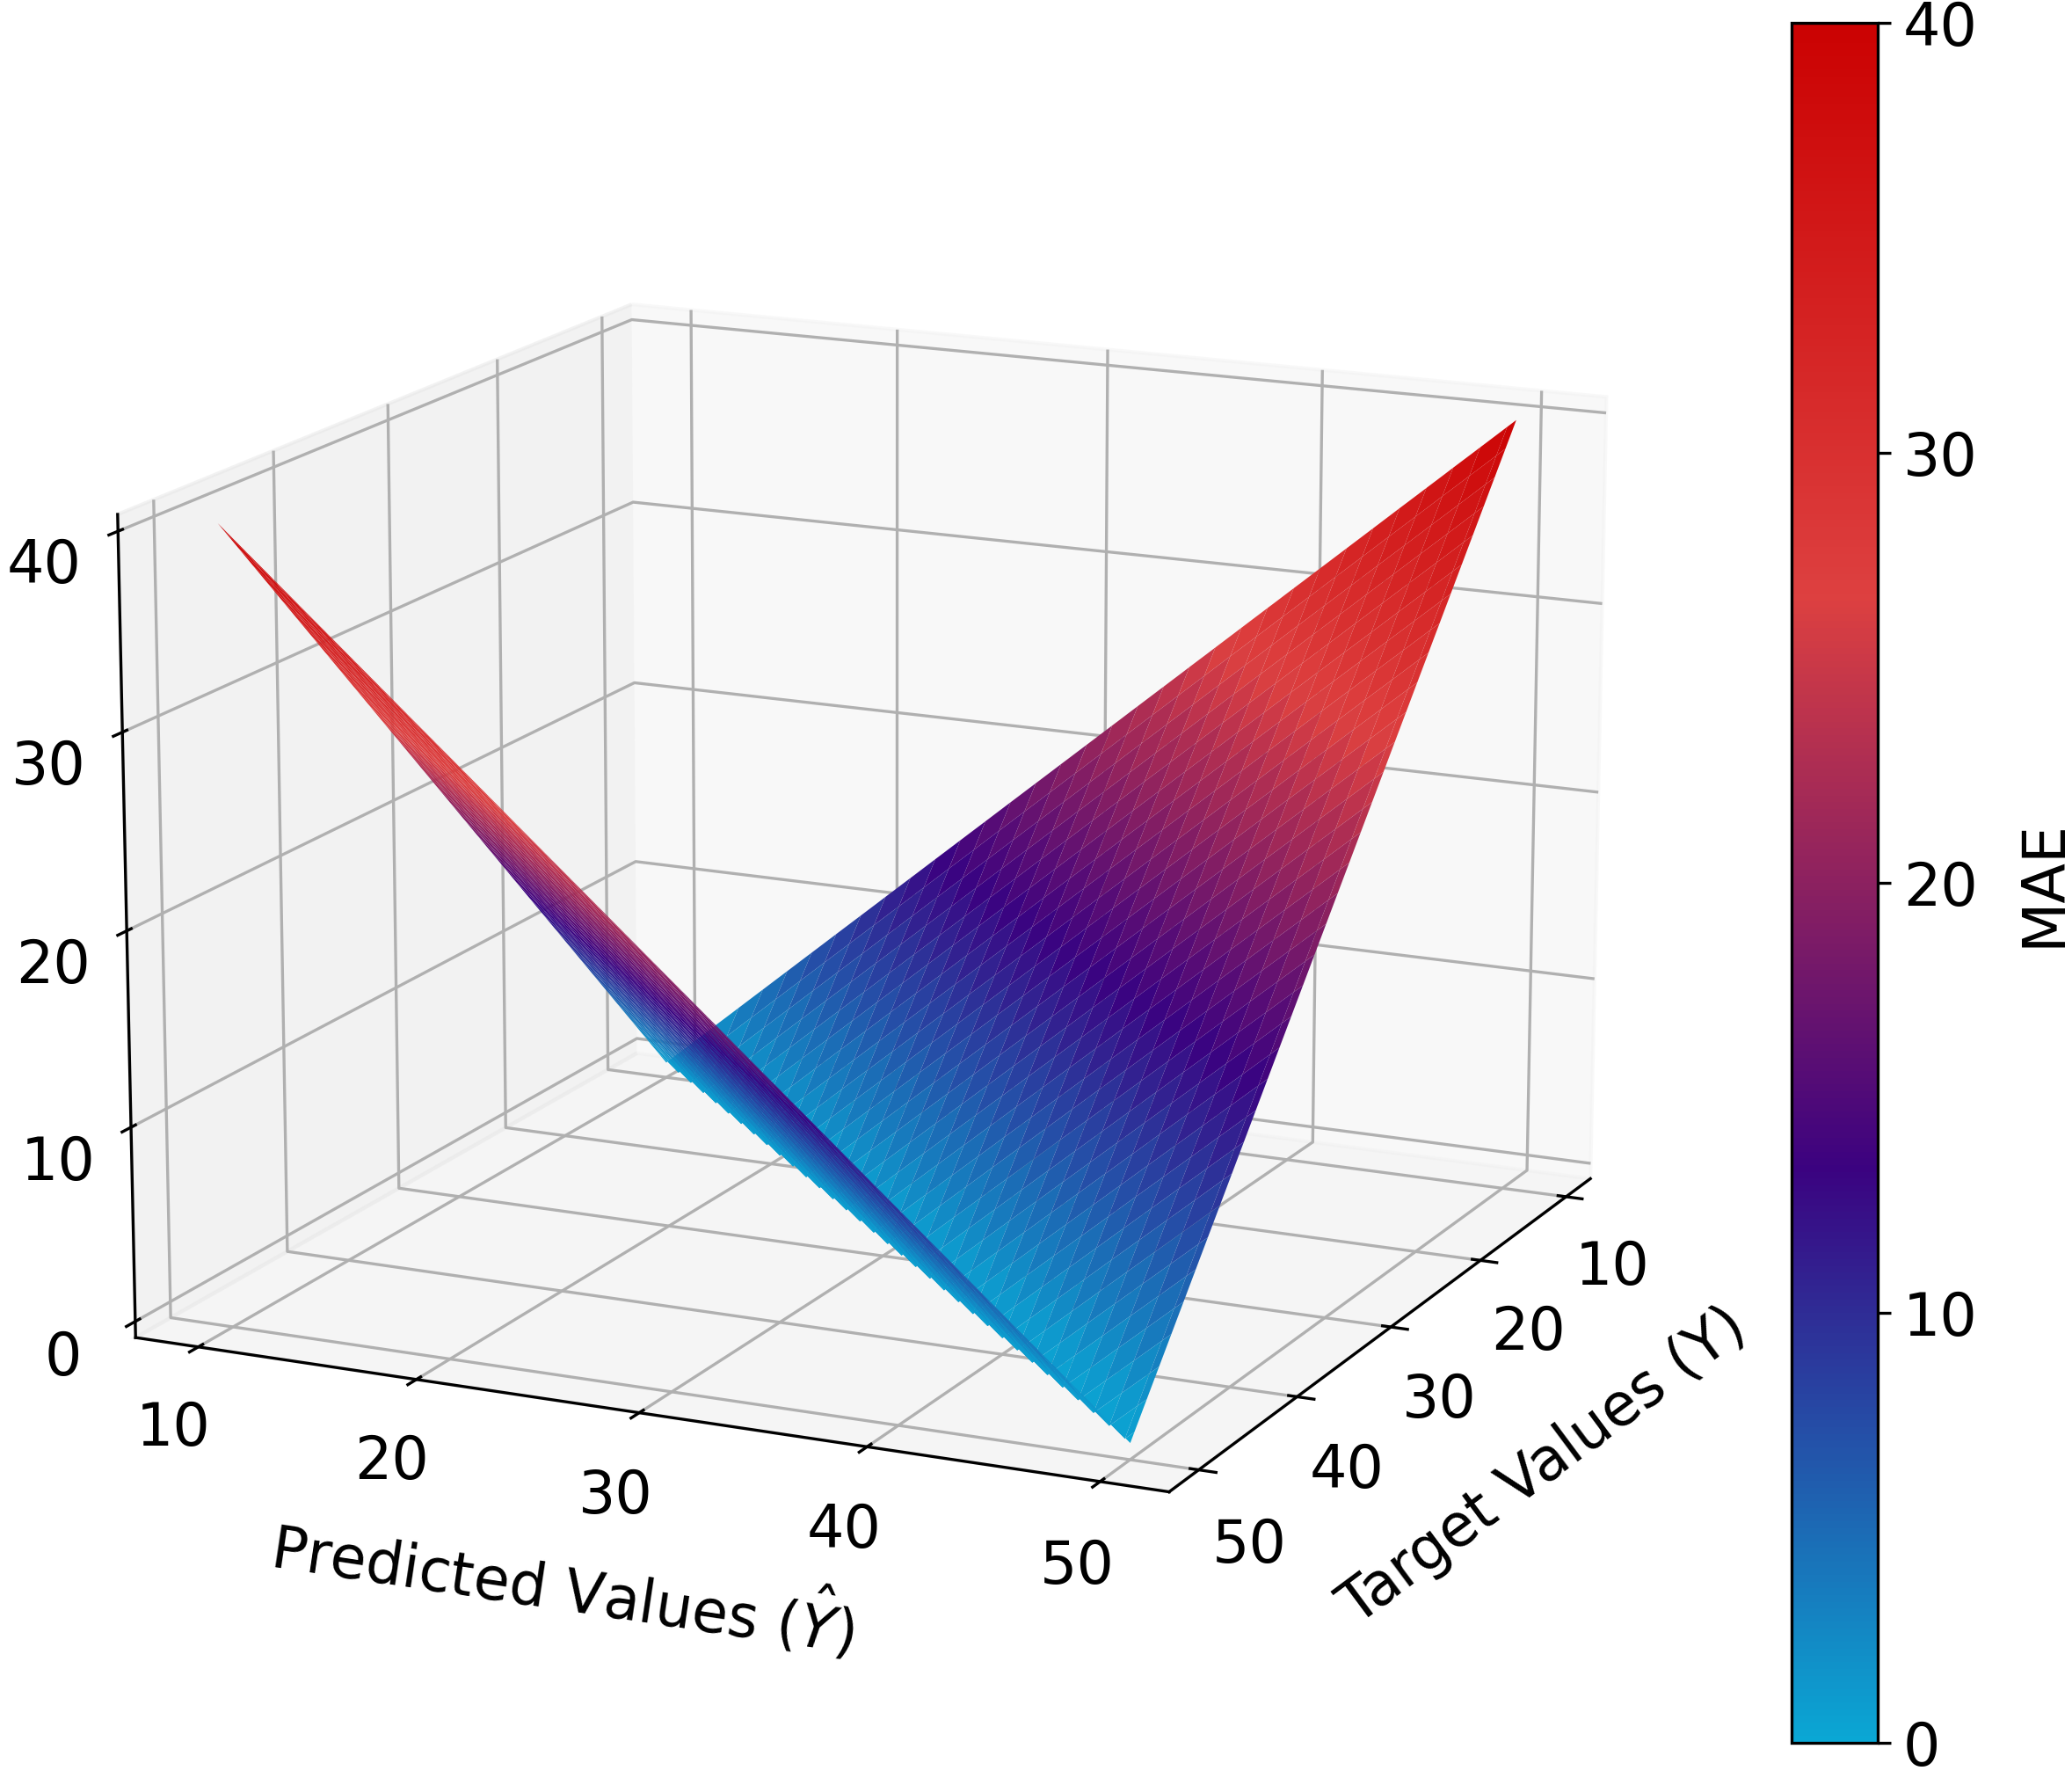
\includegraphics[width=0.6\textwidth]{figures/MAE_3d_surface.png}
    % \caption{Caption}
\end{figure*}

\begin{wrapfigure}{r}{0.5\textwidth}
    \centering
    \vspace{-10pt} % Adjust vertical alignment if needed
    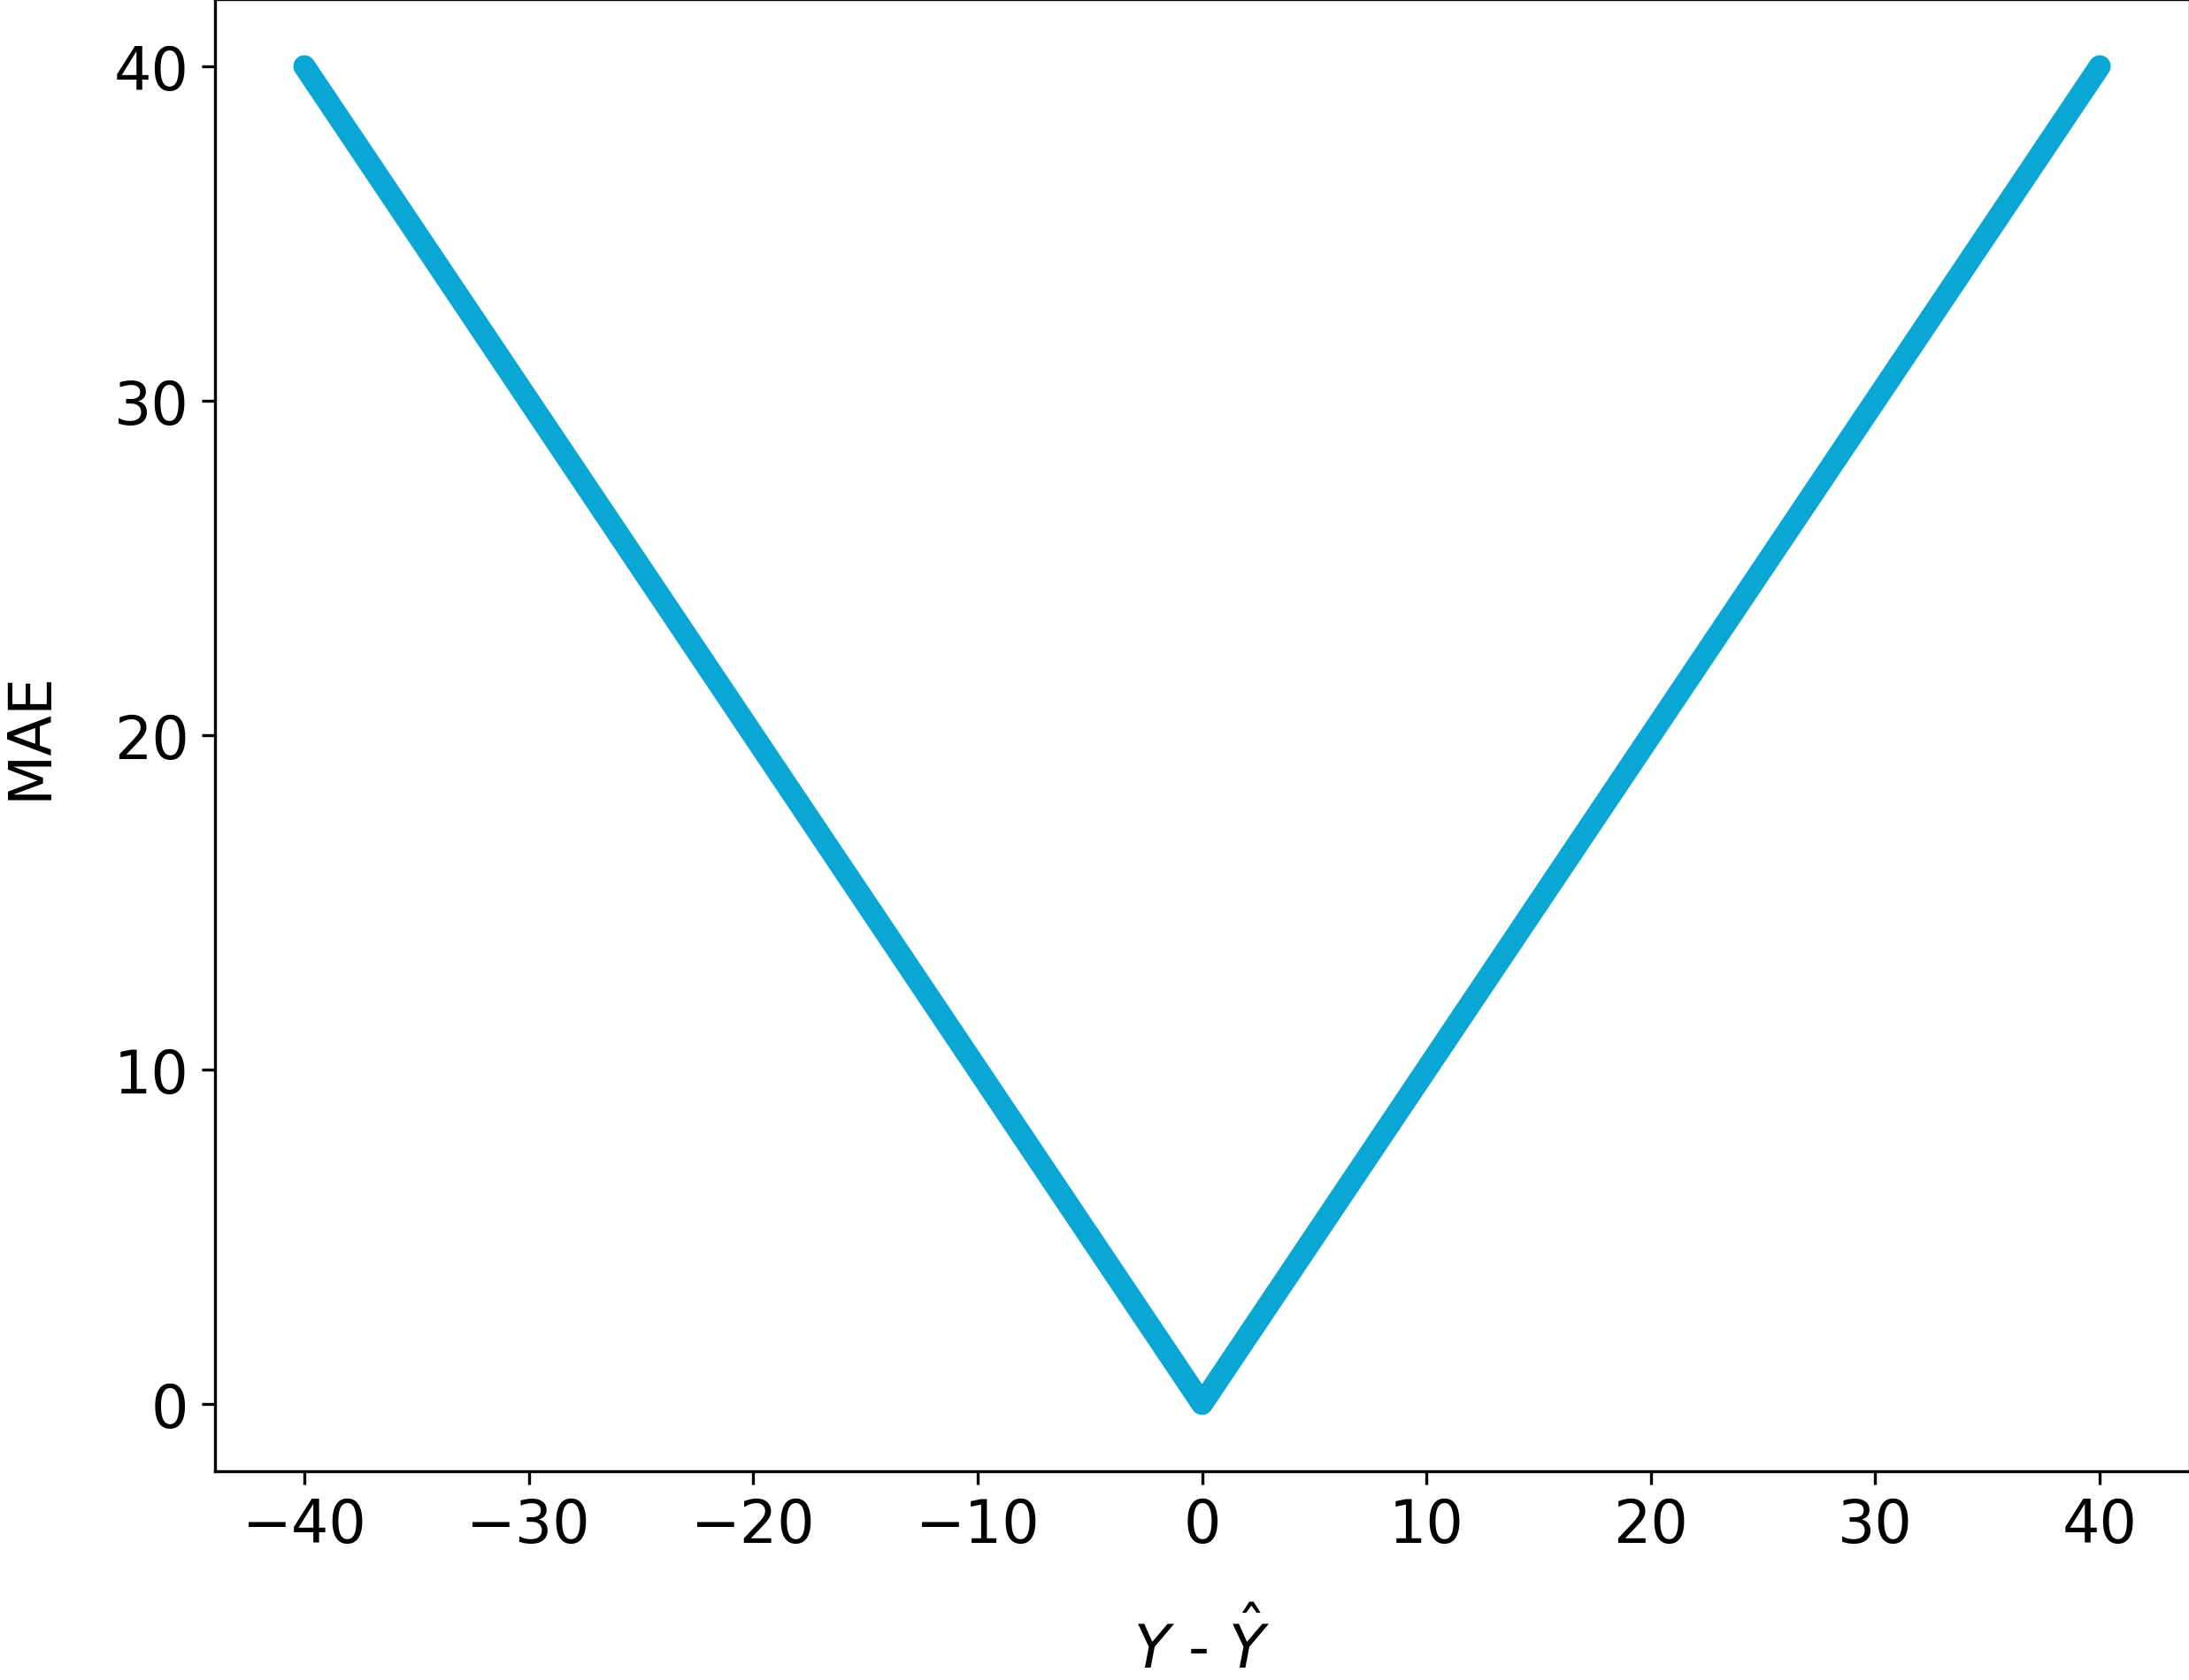
\includegraphics[width=0.45\textwidth]{figures/MAE_cross_section.png} % Your figure goes here
    \vspace{-10pt} % Adjust vertical alignment if needed
\end{wrapfigure}

% Left text with the image on the right
\textbf{Figure 2.1 MAE.} \underline{Top:} The rate of change of MAE is linear. 
Each error contributes proportionally to the total error. 
\underline{Right:} We can see that MAE is always non-negative, symmetrical,
and cantered around zero. By looking at this plot it is clear that MAE is not differentiable at zero.

\orangebox{Did you know that...}
{A forecast method that minimizes MAE
will lead to forecasts of the median.}


\textbf{Other related metrics}

Other metrics commonly explored alongside MAE are Mean Squared Error (MSE), Root Mean Squared Error (RMSE), 
and Mean Absolute Percentage Error (MAPE).

% ---------- MSE ----------
\clearpage
\thispagestyle{regressionstyle}
\section{MSE}
\subsection{Mean Squared Error}

% ---------- MSLE ----------
\clearpage
\thispagestyle{regressionstyle}
\section{MSLE}
\subsection{Mean Squared Log Error}

% ---------- RMSE ----------
\clearpage
\thispagestyle{regressionstyle}
\section{RMSE}
\subsection{Root Mean Squared Error}

% ---------- RMSLE ----------
\clearpage
\thispagestyle{regressionstyle}
\section{RMSLE}
\subsection{Root Mean Squared Log Error}

% ---------- MAPE ----------
\clearpage
\thispagestyle{regressionstyle}
\section{MAPE}
\subsection{Mean Absolute Percentage Error}

% ---------- sMAPE ----------
\clearpage
\thispagestyle{regressionstyle}
\section{sMAPE}
\subsection{Symmetric Mean Absolute Percentage Error}

% ---------- wMAPE ----------
\clearpage
\thispagestyle{regressionstyle}
\section{wMAPE}
\subsection{Weighted Mean Absolute Percentage Error}

% ---------- MASE ----------
\clearpage
\thispagestyle{regressionstyle}
\section{MASE}
\subsection{Mean Absolute Scaled Error}

% ---------- MSPE ----------
\clearpage
\thispagestyle{regressionstyle}
\section{MSPE}
\subsection{Mean Squared Prediction Error}

% ---------- MDA ----------
\clearpage
\thispagestyle{regressionstyle}
\section{MDA}
\subsection{Mean Directional Accuracy}

% ---------- MAD ----------
\clearpage
\thispagestyle{regressionstyle}
\section{MAD}
\subsection{Mean Absolute Deviation}

% ---------- MPD ----------
\clearpage
\thispagestyle{regressionstyle}
\section{MPD}
\subsection{Mean Poisson Deviance}

% ---------- MGD ----------
\clearpage
\thispagestyle{regressionstyle}
\section{MGD}
\subsection{Mean Gamma Deviance}

% ---------- R-squared ----------
\clearpage
\section{$\mathbf{R^2}$}
\subsection{R-squared}
\thispagestyle{regressionstyle}

R-squared needs little introduction; it's featured in every statistics book. Also known as the coefficient of determination, it's commonly introduced as a measure that quantifies the amount of variability explained by the regression model.

\begin{center}
    \tikz{
        \node[inner sep=2pt, font=\Large] (a) {
            {
                $\displaystyle
                R^2 = 1 - \frac{\sum_{t=1}^n (Y_t - {\color{nmlpurple}\hat{Y}_t})^2}{\sum_{t=1}^n ({\color{nmlcyan}Y_t} - {\color{teal!70!green}\bar{Y}})^2}
                $
            }
        };
        
        \draw[-latex,nmlpurple, semithick] ($(a.north)+(2.1,0)$) to[bend left=15] node[pos=1, right] {Predicted value} +(1,.5); 
        \draw[-latex,teal!70!green, semithick] ($(a.south)+(2.1,0.1)$) to[bend right=15] node[pos=1, right] {Mean of targets} +(1,-.5); 
        \draw[-latex,nmlcyan, semithick] ($(a.south)+(1,0.1)$) to[bend left=15] node[pos=1, left] {Target value} +(-1,-.5); 
    }
\end{center}

However, it may be easier to think of R-squared as a way to scale MSE between a perfect model and one that always predicts the mean. A score of 1.0 means $Y_t$ and $\hat{Y}_t$ are equal. Despite its name, R-squared can be negative if the model performs worse than just predicting the mean.

\textbf{When to use R-squared?}

R-squared can be more intuitive than MAE, MSE, RMSE, and other scale-dependent metrics since it can be expressed as a percentage, whereas the latter have arbitrary ranges.

\coloredboxes{
    \item Easy Interpretation. Especially when interpreted as a scaled MSE.
    \item R-squared is widely accepted in statistical analysis and research, making it a standard choice for evaluating model performance.
}
{
    \item Just like MSE, R-squared can be sensitive to outliers, as large errors have a greater impact.
    \item Be cautious about which value of $\bar{Y}$ to use. Most implementations default to $\bar{Y}_{\text {test }}$ which can lead to information leakage. It is advisable to use $\bar{Y}_{\text {train }}$ instead.
}


\clearpage
\thispagestyle{customstyle}


\begin{figure*}[ht!]
    \centering
    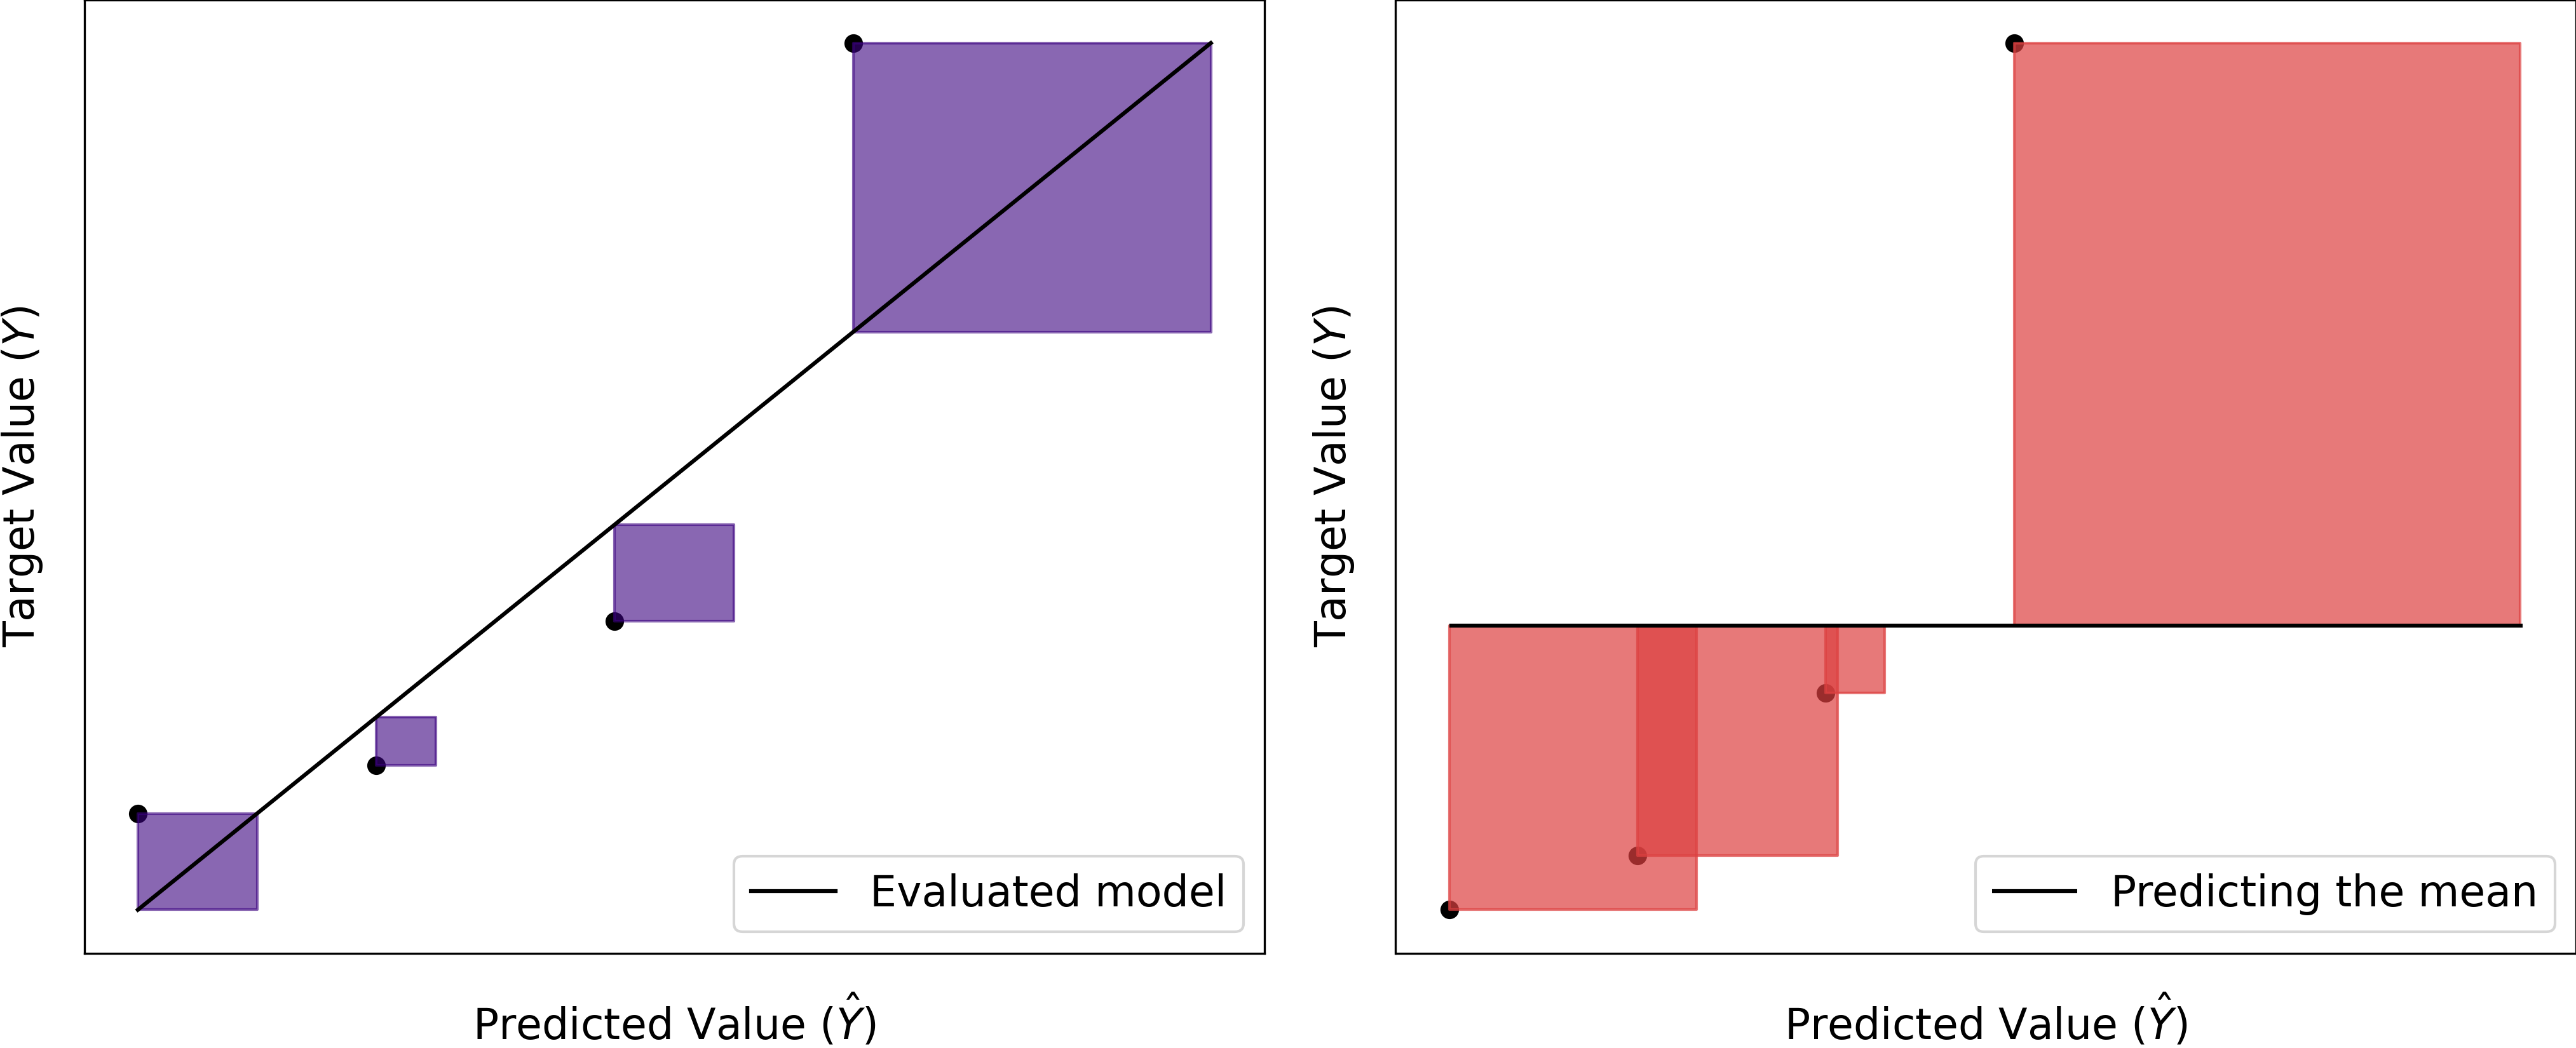
\includegraphics[width=\textwidth]{figures/R2_explained.png}
    % \caption{Caption}
    \label{fig1}
\end{figure*}

\begin{wrapfigure}{r}{0.5\textwidth}
    \centering
    \vspace{-10pt} % Adjust vertical alignment if needed
    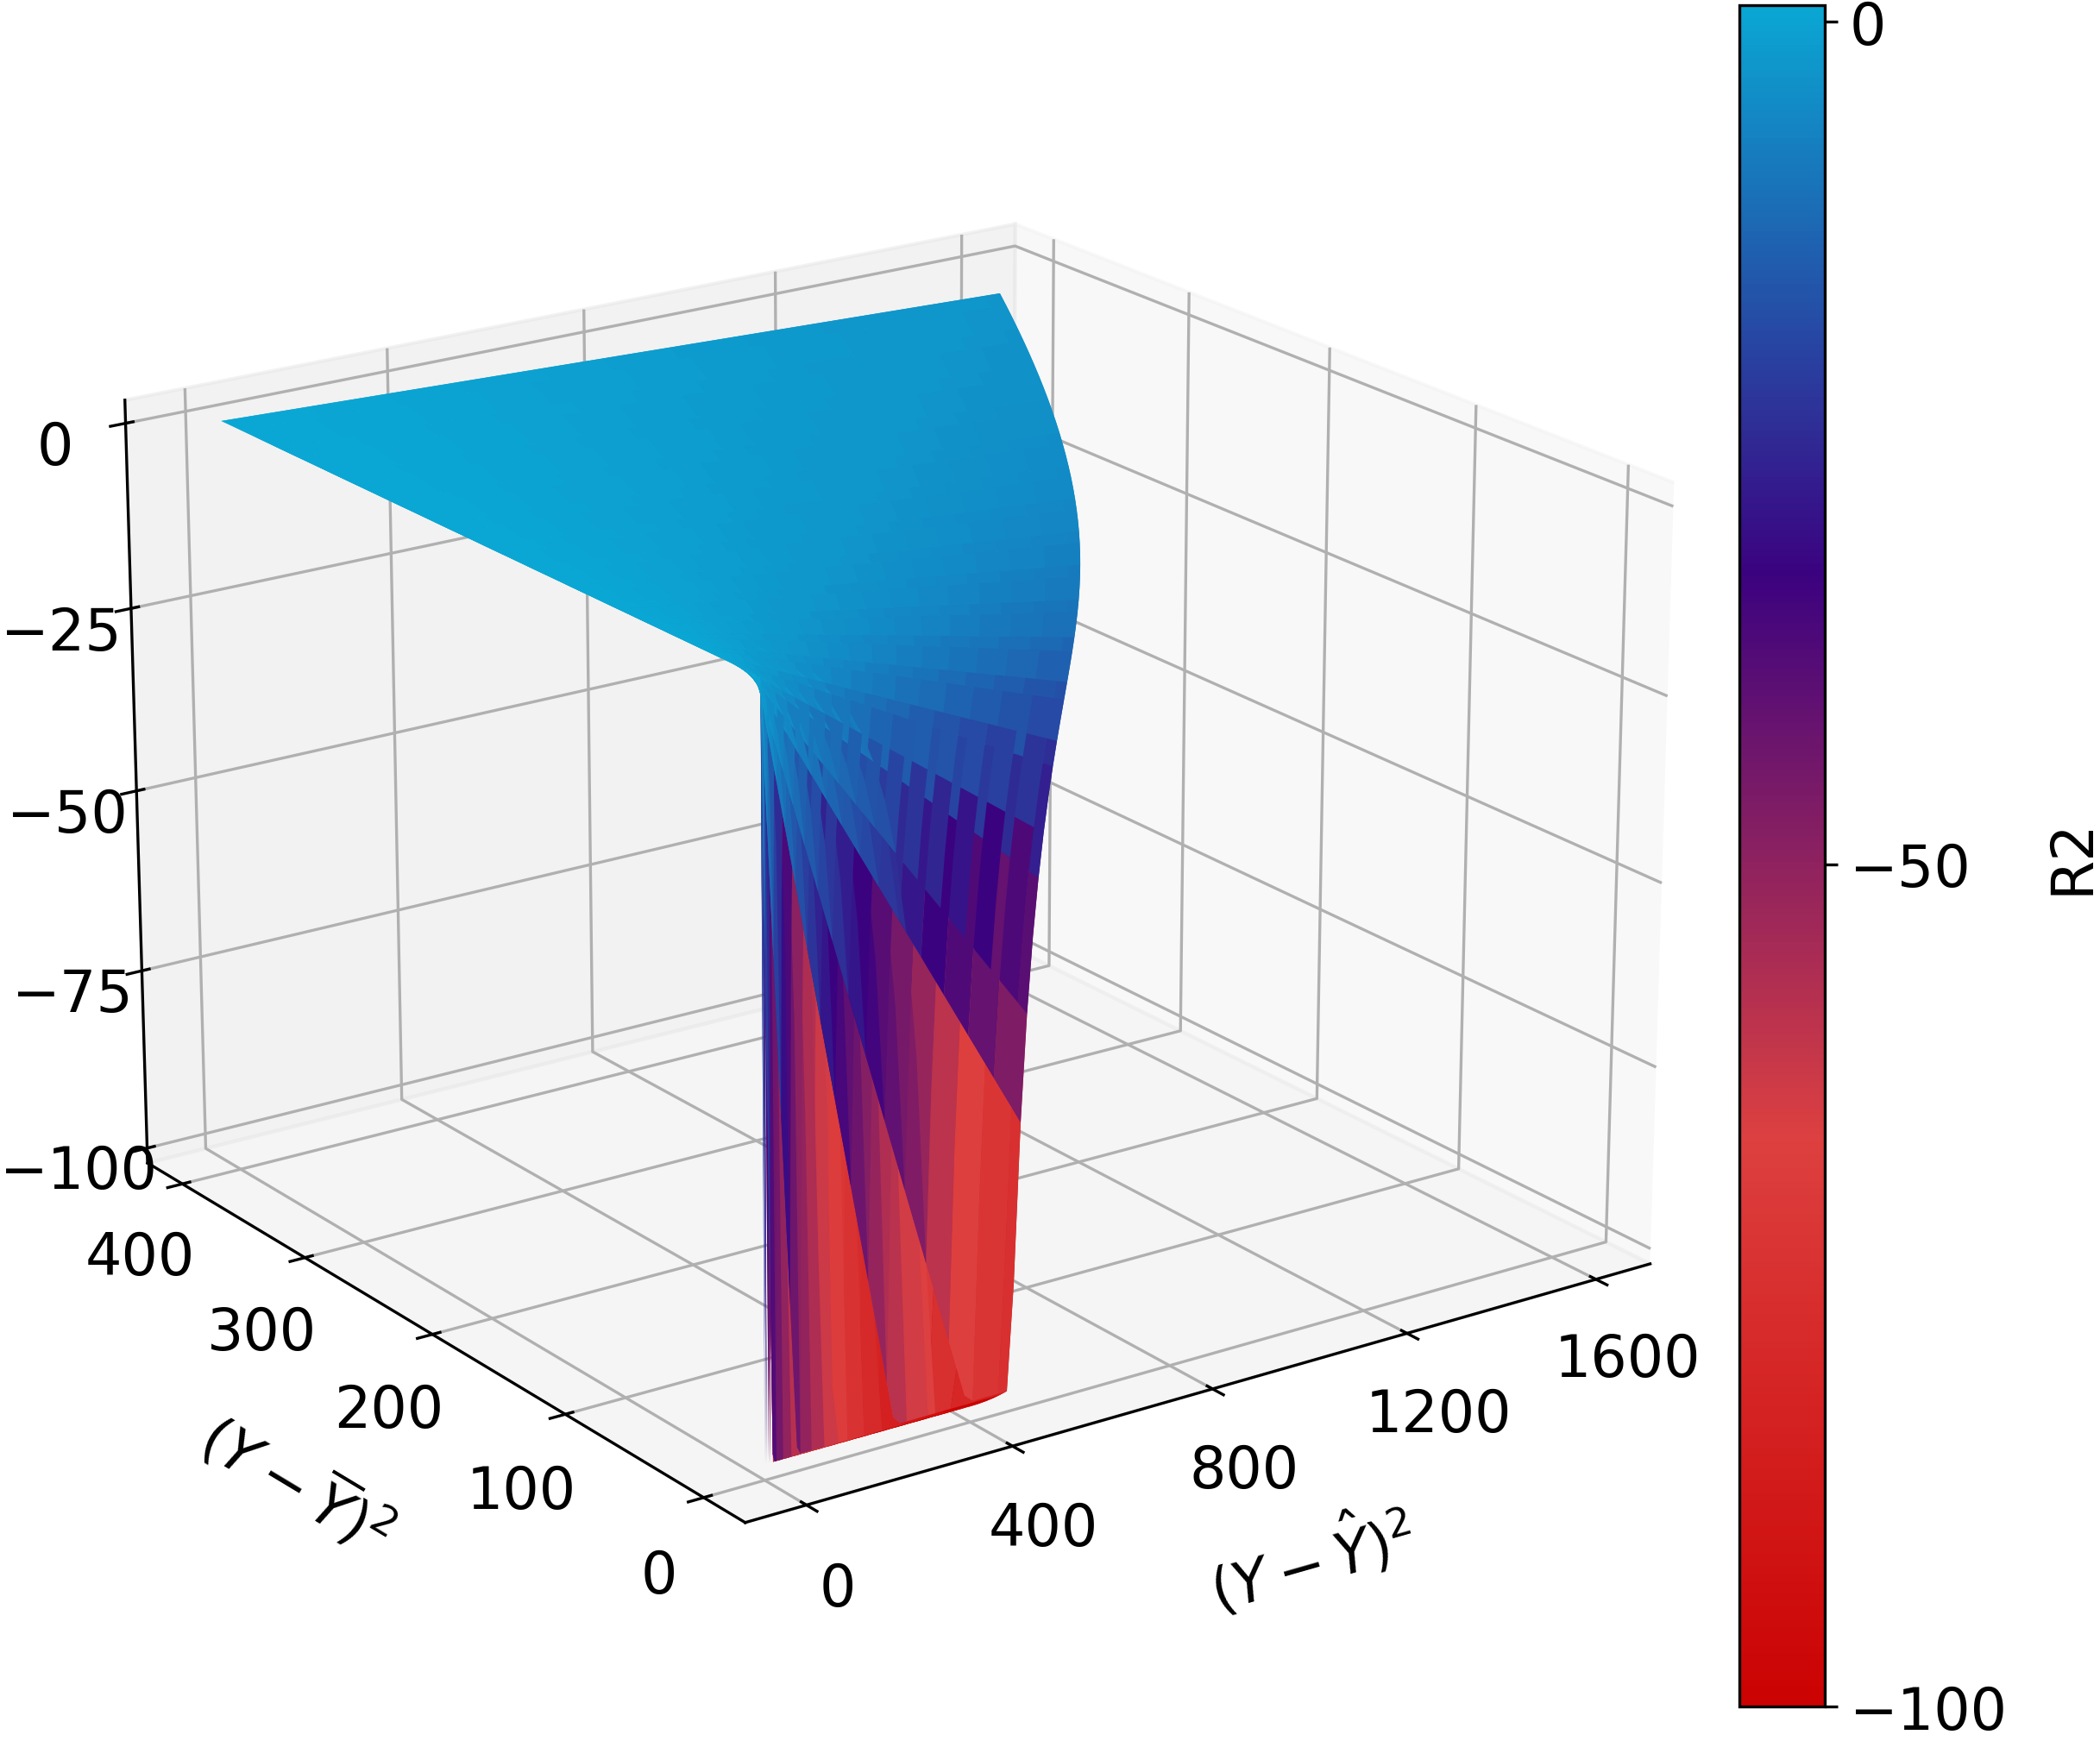
\includegraphics[width=0.45\textwidth]{figures/R2_3d_surface.png} % Your figure goes here
    \vspace{-10pt} % Adjust vertical alignment if needed
\end{wrapfigure}

% Left text with the image on the right
\textbf{Figure 2.15 R-Squared.} \underline{Top:} The
areas of the purple squares
represent the MSE of the
evaluated model. While, the areas
of the red squares represent the
MSE of a model that always
predicts the mean. R-squared
can be written as $R^2 = 1-\frac{\color{violet!50}MSE_{model}}{\color{nmlred}MSE_{baseline}}$\\
\underline{Right:} R-squared quickly drops
into the negative region in cases
where the mean is a better
predictor than the evaluated
model.


\orangebox{%
Did you know that...}
{
R-squared is more than 100 years old; it was introduced by geneticist Sewall Wright in 1921.
}


\textbf{R-squared alternatives and related metrics}

Other metrics commonly explored alongside R-squared are Adjusted Rsquared, out-of-sample R-squared,
Mean Absolute Error (MAE), Mean Squared Error (MSE), Root Mean Squared Error (RMSE), etc.



% ---------- D2 ----------
\clearpage
\thispagestyle{regressionstyle}
\section{D2}
\subsection{D2 Absolute Score}

% ---------- Explained Variance Score ----------
\clearpage
\thispagestyle{regressionstyle}
\section{Explained Variance Score}
\subsection{Explained Variance Score}